\documentclass[compress]{beamer}
\usepackage{graphicx}
\usepackage{enumerate}
\usepackage{amssymb}
\usepackage{cancel}
\usepackage[utf8]{inputenc}
\usepackage{color}
\usepackage{dcolumn}
\newcolumntype{d}[1]{D{.}{.}{#1}}
\usepackage[francais]{babel}
\usepackage{tikz}
\usepackage{soul}
\newcommand{\esN}{\mathbb{N}}
\newcommand{\esR}{\mathbb{R}}
\usetheme[navigation]{UMONS}
\setbeamertemplate{caption}[numbered]
\title{Analyse en composantes indépendantes}
\date{25 mai 2016}
\author[G. \textsc{Huysmans}, M. \textsc{Lempereur}]
	{Guillaume \textsc{Huysmans}, Martin \textsc{Lempereur}}
\institute[]{Département d'Informatique \\
	Université de Mons \\[2ex]
\includegraphics[height=4ex]{UMONS}\hspace{2em}
	\raisebox{-1ex}{
\includegraphics[height=6ex]{UMONS_FS}}}
\bibliographystyle{plain}
\begin{document}
\begin{frame}
	\maketitle
\end{frame}
\begin{frame}
	\frametitle{Plan}
	\tableofcontents
\end{frame}


\section{Résumé théorique}
\begin{frame}
	\frametitle{Problème de la soirée cocktail}
	Plusieurs micros $x_i$ sont disposés parmi
	différentes personnes $s_j$ qui parlent en même temps.
	L'objectif est de calculer une approximation de $s_j$
	ainsi que la matrice de mixage $A$ afin que $AS=X$.

	\begin{block}{Linéarité}
	Ainsi, nous ferons l'hypothèse que chaque micro capture
	une combinaison linéaire de ce que les gens (sources) émettent :
	\[
		\forall i\in\esN \qquad x_i = \sum_{j=0}^k a_{ij} s_j
	\]
	\end{block}
	\pause

	Si nous disposions de $A$, le problème serait simple :
	\[
		\cancel{(A^{-1}A)}S = A^{-1}X
	\]
\end{frame}

\begin{frame}
	\frametitle{Exemple numérique}
	\[
		\underbrace{\left(\begin{array}{lll}
			1 & 1 & 1 \\
			\color{red}1 & \color{red}3 & \color{red}1 \\
			3 & 1 & 0
		\end{array}\right)}_{\text{A }(3\times3)}
		\underbrace{\left(\begin{array}{ccccc}
			0 & 1 & \color{green}2 & 3 & 4 \\
			5 & 5 & \color{green}0 & 5 & 5 \\
			1 & -1 & \color{green}1 & -1 & 1
		\end{array}\right)}_{\text{S }(3\times5)}=
		\underbrace{\left(\begin{array}{rrrrr}
			6 & 5 & 3 & 7 & 10 \\
			16 & 15 & \color{blue}3 & 17 & 20 \\
			5 & 8 & 6 & 14 & 17
		\end{array}\right)}_{\text{X }(3\times5)}
	\]

	Chaque ligne $\color{red}a_i$ (coefficients pour le micro $i$) est multipliée
	par une~colonne $\color{green}s_j$ (échantillons-sources en $t=j$)
	afin d'obtenir l'{\color{blue}amplitude} mesurée
	par le~micro $i$ en le temps $j$.
	$X$ contient ainsi un vecteur-ligne par micro.
	\pause

	On peut retrouver $S$ à partir de $A$ et de $X$ (c'est équivalent à la
	résolution d'un système d'équations linéaires) :
	\[
		S\approx
		\left(\begin{array}{d{3.1}d{3.1}d{3.1}}
			0.17 & -0.17 & 0.33 \\
			-0.50 & 0.50 & 0 \\
			1.33 & -0.33 & -0.33
		\end{array}\right)
		\left(\begin{array}{rrrrr}
			6 & 5 & 3 & 7 & 10 \\
			16 & 15 & 3 & 17 & 20 \\
			5 & 8 & 6 & 14 & 17
		\end{array}\right)
	\]
\end{frame}

\begin{frame}
	\frametitle{Limites}
	À cause de la structure du problème, une technique de résolution,
	quelle qu'elle soit, ne permettra pas de tout déterminer :
	\pause
	\begin{enumerate}
	\item L'ordre des sources ne peut pas être déterminé.
	\pause
		\\\textit{Intuition : l'addition est commutative et nous n'avons que
			des sommes pondérées à disposition.}
	\pause
	\item L'amplitude absolue des sources ne peut pas être déterminée.
	\pause
		\\Une source atténuée peut être amplifiée au mixage :
			multiplier une~colonne de $A$ par $k\in\esR_0$ et
			diviser une ligne de $S$ par celui-ci ne change rien à
			la valeur de $X$.
	\pause
	\end{enumerate}

	Ces informations ont en fait été perdues lors du mixage.
\end{frame}
\begin{frame}
	\frametitle{Pré-traitement des données}
	L'algorithme de FastICA demande en entrée des données qui sont traitées.
	Deux opérations doivent être exécutées sur les données :
	\pause
	\begin{enumerate}
	\item Blanchissement des données.
		\pause
			\\Le blanchissement des données est une
			technique\footnote{Utilisée aussi pour l'ACP}
			qui consiste à décorréller les données en diagonalisant
			leur matrice de covariance.
	\pause
	
	\end{enumerate}
\end{frame}
\begin{frame}
	\frametitle{Gaussianité}
	Pour pouvoir faire apparaître des structures plus intéressantes,
	on va vouloir projeter les données sur un espace de faible dimension.
	Le but est d'éloigner les nuages de points les uns des autres.
	Pour y arriver, on va essayer de s'éloigner du cas de données gaussiennes.
	On va minimiser ce qu'on appelle la \textit{néguentropie} :
	plus cette valeur est petite, moins la distribution des données
	est gaussienne.
\end{frame}


\section{Implémentation}
\begin{frame}
	\frametitle{FastICA}
	Le mixage est modélisé dans l'autre sens :
	\[
		S^TA^T=X^T
	\]
	%TODO match the doc
\end{frame}


\section{Exemples}
\begin{frame}
	\frametitle{Sinusoïdes}
	Un des cas les plus simples est la superposition de sinusoïdes.
	\vfill

	\begin{minipage}[b]{.35\textwidth}
	\begin{figure}[h]
	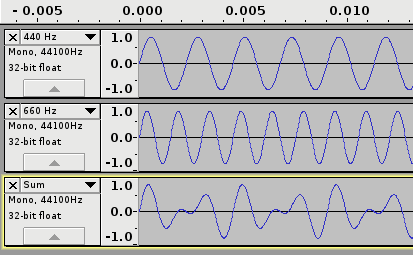
\includegraphics[width=\textwidth]{sine.png}
	\caption{Avant}
	\end{figure}
	\end{minipage}
	\hfill
	\begin{minipage}[b]{.35\textwidth}
	\begin{figure}[h]
	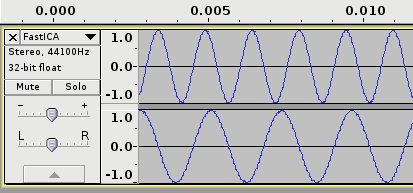
\includegraphics[width=\textwidth]{sine_d.png}
	\caption{Après}
	\end{figure}
	\end{minipage}

	\begin{block}{Observation}
	L'ordre n'est pas préservé et lors de cette exécution,
	la sinusoïde à 660~Hz arrive la première dans le résultat.
	\end{block}
\end{frame}


\begin{frame}
	\frametitle{Extraits audio}
	Deux extraits très différents sont joués en même temps.
	On les suppose indépendants et non gaussiens...
	\begin{figure}[h]
	\includegraphics<1>[height=.65\textheight]{blunt_kavinsky_r.png}
	\includegraphics<2>[height=.65\textheight]{blunt_kavinsky_l.png}
	\includegraphics<3>[height=.65\textheight]{blunt_kavinsky_m2.png}
	\caption{
		\only<1>{James Blunt - Postcards}
		\only<2>{Kavinsky - Night Call}
		\only<3>{\st{Mix} Superposition}
	}
	\end{figure}
\end{frame}


\appendix
\begin{frame}
	\frametitle{Références}
	La théorie est un résumé de l'article suivant :
	\bibliography{article}
	\vspace{2em}

	Le module R utilisé est
	\href{https://cran.r-project.org/web/packages/fastICA/}{FastICA},
	développé par J.~L.~Marchini, C.~Heaton et B.~D.~Ripley et
	se base également sur \cite{hyv}.
\end{frame}


\end{document}
